\chapter{Passive Dynamics of Legged Locomotion}
\label{sec:PassiveDynamicsOfLeggedLocomotion}
\index{passive dynamics}

In section \ref{sec:SLIP} it was said that the SLIP locomotive could achieve
stable motion if initial conditions are appropriate. The fact that such motion
can sustain itself without any active feedback or input (an isolated system)
means the motion is passively stable. Thus, it may be possible to achieve
locomotion passively. This has various implications, especially for the design
of efficient (and thus more human-like) walking robots \cite{collins}. To build
up to an analysis of passive SLIP motion, we first examine the passive 2D
motion of a rimless wheel rolling down an incline.


%%%%%%%%%%%%%%%%%%%%%%%%%%%%%%%%%%%%%%%%%%%%%

% I just put this section here from the "introduction to stability" It may be spread around to other places. 

\section{Introduction to Stability} % (notes page 20-26)
\label{sec:IntroductionToStability}
\index{stability}

Understanding the passive dynamics of the models presented in Chapter
\ref{sec:ModelingLeggedLocomotion} requires a basic understanding of the
concept of stability. We consider locomotion to be a stable periodic motion of
a dynamic system, where the dynamic system is defined by ordinary differential
equations and sometimes collision equations. The motion of a dynamic system is
considered to be stable when the system is capable of rejecting disturbances.
A legged animal or robot that is moving with a stable gait, given some
perturbation in its motion, will return to the motion it was performing before
the perturbation was introduced. Experiment and theory have both shown that
certain legged animals and robots can walk or run with a stable motion without
any control; the motion is passively stable. We will see later on that the
mathematical description for such motion is a stable fixed point on a Poincare
section or map. 

% FIGURE
\begin{figure}[h]		% h="here" t="top" b="bottom" p="separate page"
\begin{centering}
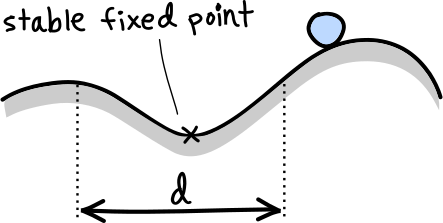
\includegraphics[width=0.55\textwidth]{Figures/BallOnHill}\par
\end{centering}
\caption[Diagram: Ball in a Valley]{Ball in a valley. If the ball is released
from the hill to the right at a height that is no greater than that of the hill
to the left, the ball will remain in the valley between hills. After some time,
the ball comes to rest at the stable fixed point at the bottom of the valley.
The steady state position of the ball can also be thought of as periodic motion
in which the ball is found at the stable fixed point at the end of each period
of the motion. This periodic motion mindset is useful for locomotion models.}
\label{fig:BallOnHill}
\end{figure}
%

Imagine a system like the one shown in figure \ref{fig:BallOnHill}: two hills,
with a valley between them, and a ball that starts on the side of the larger
hill. Imagine that the interaction between the ball and the hill is \emph{not}
frictionless, but the rolling resistance is small. When the ball is released,
it rolls left down the hill, passing by the lowest point in the valley,
and rolls over the peak of the smaller hill. Now imagine the ball starts a
little bit lower on the side of the larger hill, such that it rolls through the
valley, and does not roll past the peak of the smaller hill. It reaches some
maximum height, and rolls back the way it came. The ball oscillates back and
forth until it comes to rest at the bottom of the valley. 

Though slightly un-intuitive, one can think of the motion of the ball as
periodic in time. When the ball is resting at the bottom, we consider the ball
to be in ``motion," where the period of the motion is infinitesimal. The
resting point is considered a stable fixed point, because for every period of
the motion, the ball returns to that point. If the ball's ``motion" is
disturbed by an external force, after some number of periods it will return to
the stable fixed point. In this case, it is a little silly to think of it that
way, because between periods, the ball is still at stable fixed point during
its ``motion." \todo[inline]{get rid of previous sentence?} The path that it
follows along the hill as it settles to that fixed point can be thought of as
the basin of attraction: if the ball starts anywhere in the basin, it reaches
the stable fixed point. 

In the case of the ball in figure \ref{fig:BallOnHill}, the basin of attraction
is two-dimensional. The ball can be assumed to be on the surface of the hill,
and its state can be described by two parameters: position along the path, and
velocity in the direction of travel. A Poincare map is a visualization of these
two parameters sampled once per period, in two-dimensional space, as in figure
\ref{fig:BasinOfAttraction}. Parameters like position and velocity can be
assigned to the $x$ and $y$ axes of the Poincare map, and the stable fixed
point can be located on the map. Figure \ref{fig:BasinOfAttraction} is a
generalized version of a Poincare map. In the case of the ball on the hill, the
stable fixed point would be at position $y = 0$ and velocity $x = 0$. A general
fixed point is marked with a star on the map, as shown in figure \ref{fig:BasinOfAttraction}. 

% FIGURE
\begin{figure}[h]		% h="here" t="top" b="bottom" p="separate page"
\begin{centering}
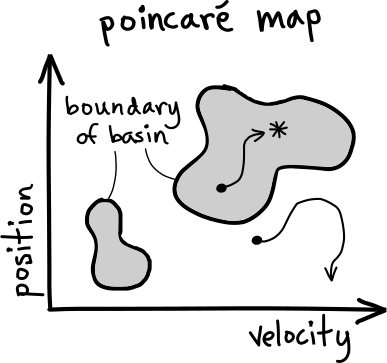
\includegraphics[width=0.3\textwidth]{Figures/BasinOfAttraction}\par
\end{centering}
\caption[Diagram: Poincare Map with Basins of Attraction]{Poincare map with basins of attraction. The map, drawn here for a general system, has coordinates of position and velocity. Points on the map denote the position and velocity state of a system at the end of each period of the system's motion. Basins of attraction are shaded, and fixed points are labeled as stars. If the initial state of a system, denoted as a dot, is within a basin of attraction, the system will tend toward the fixed point contained in that basin. If the initial state lies outside a basin, its configuration in time does not tend toward a particular steady motion.}
\label{fig:BasinOfAttraction}
\end{figure}
%

\todo[inline]{can there be a basin of attraction without a fixed point, as is
shown in the figure?}

The basin of attraction is made up of all the states (position and velocity)
that the ball or system can have initially and still return to the stable fixed
point. In the ball example, it's important to note that the ball may start in
the region $d$ shown in figure \ref{fig:BallOnHill}, but if the velocity is
nonzero and too great, the ball may not ever reach the stable fixed point. 

The stable fixed point is generally called an attractor, and up to this point we've been thinking of the attractor as one point on the Poincare map. However, it is also possible that the attractor could be a complicated region. These complicated regions are sometimes called ``strange attractors." Functionally, strange attractors are the same as a stable fixed point. If the state of the system lies within the attractor, it will return to somewhere else within that attractor one period later, just as a system would return to the stable fixed point one period later. figure \ref{fig:Attractors} shows the difference between the two attractors.

% FIGURE
\begin{figure}[h]		% h="here" t="top" b="bottom" p="separate page"
\begin{centering}
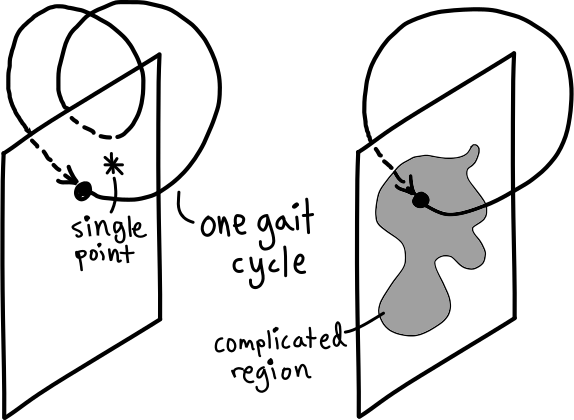
\includegraphics[width=0.5\textwidth]{Figures/Attractors}\par
\end{centering}
\caption[Diagram: Single Point Attractors and Strange Attractors]{Single point attractors and strange attractors. The left Poincare section is for a single point attractor, denoted by the star. The right Poincare section is for a strange attractor, where the shaded area is the strange attractor. If the system's state is within an attractor region, the system's state at the end of all periods will lie within the attractor. Note that the basin of attraction is not shown for either attractor. The strange attractor on the right could be enclosed by a larger basin of attraction. If a disturbance is introduced that doesn't move the trajectory outside the basin of attraction, the trajectory will return to the complicated region after some time.}
\label{fig:Attractors}
\end{figure}
%

The section shown on the left of figure \ref{fig:Attractors} is an example of a
single point attractor, showing what might happen if a disturbance is
introduced. The trajectory traced around the section shows that the motions are
periodic, and do not quite pass through the stable fixed point on each period.
As long as the trajectory of the state passes through the basin of attraction,
the trajectory of the state will return to the stable fixed point, and become a
single loop like the section shown on the right. 

As may be apparent from the previous two figures, much of our analysis of stability is rooted in the state-space representations of systems. In such a representation, there is a state that the robot is operating at, if you introduce a disturbance to the state, perhaps $\epsilon$, we want to know if the state space representation returns to what it was before the disturbance was introduced. More tools for analyses like these can be found in books on feedback control, such as Ogata \cite{ogata09} (Root Locus, Nyquist, etc). These tools will not be used extensively in this chapter, but understanding the reasons for their use in other systems will be helpful to understanding stability analyses of legged locomotion models. 

%%%%%%%%%%%%%%%%%%%%%%%%%%%%%%%%%%%%%%%%%%%%

\section{Rimless Wheel} % (notes page 20-26)
\label{sec:RimlessWheel}
\index{rimless wheel dynamics}

The motion of a rimless wheel is a classical problem that exhibits some basic aspects of passive stable motion and permits a nice introduction to examining the stability of locomotion models. Consider the rimless wheel in figure \ref{fig:RimlessWheel}, with massless spokes and a mass $m$ at its center, that is rolling down an incline $\gamma$ under the force of gravity along $\ul$. The wheel has $N$ spokes of length $l$, and each spoke is separated from the next by an angle $\phi$. The moment of inertia of the wheel about its center $G$ is $I$. The angle between the incline's normal and the spoke that is in contact with the incline is $\theta = \theta(t)$. The wheel pivots without slip about the end of this spoke, at point $C$. While pivoting, the wheel's center of mass undergoes a motion that can be described as \textit{unstable falling} \cite{coleman96}. This smooth motion occurs in between the plastic collisions of the spokes with the incline.

% FIGURE
\begin{figure}[h]		% h="here" t="top" b="bottom" p="separate page"
\begin{centering}
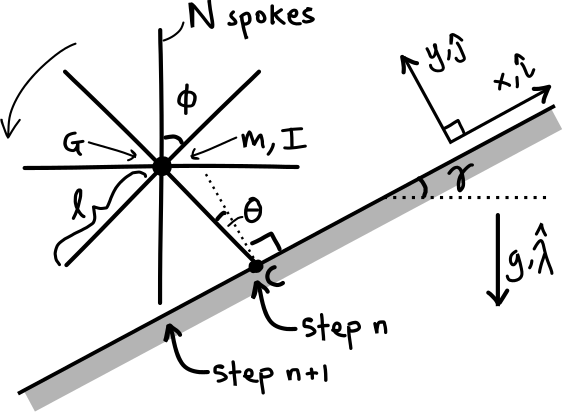
\includegraphics[width=0.6\textwidth]{Figures/RimlessWheel}\par
\end{centering}
\caption[Diagram: Rimless Wheel]{Rimless wheel. A rimless spoked wheel rotates down an incline with slope $\gamma$. The $N$ massless spokes of length $l$ are separated equally by $\phi$ degrees. The mass $m$ is located at the center of the wheel, and the wheel has moment of inertia $I$. The orientation of the wheel is specified by the angle $\theta$ that the spoke contacting the incline makes with the incline's normal.}
\label{fig:RimlessWheel}
\end{figure}
%

The objective with the rimless wheel is to compute its motion, given the parameters above. The motion has two portions: smooth motion and collisions. The motion is most likely (but not necessarily) periodic, so these two portions repeat again and again.

\textbf{Smooth ``flight":} The velocity of the mass is continuous between collisions. Angular momentum balance is a natural choice for finding the motion, since angular momentum balance about point $C$ does not include the undesired unknown of the reaction force at $C$. Using the free body diagram in figure \ref{fig:RimlessSmoothAndCollision}a,

\begin{align}
\Sigma \vec{\mathbf{M}}_{/C} &= \dot{\vec{\mathbf{H}}}_{/C} \notag \\
l \hat{\mathbf{e}}_r \times mg \ul &= \vec{\mathbf{r}}_{G/C} \times m\vec{\mathbf{a}}_G + I \dot{\omega} \hat{\mathbf{k}}
\label{eq:RimlessAMB}
\end{align}

where $\hat{\mathbf{e}}_{r}$ is a unit vector pointing from the contact point $C$ to the center of mass of the wheel $G$. The unit vectors in equation \ref{eq:RimlessAMB} can be written explicitly, and the acceleration can be written in polar coordinates.

\begin{align}
\hat{\mathbf{e}}_{r} &= - \sin{\theta} \ui + \cos{\theta} \uj \\
\ul &=  - \sin{\gamma} \ui - \cos{\gamma} \uj \\
\va_{G} &= l \thetaddot \ueth - l \thetadot^{2} \uer
\end{align}

After substituting these expressions into equation \ref{eq:RimlessAMB}, employing the trigonometric sine sum identity and performing some additional algebra, we arrive at a system of two first-order nonlinear differential equations that can be solved perhaps with a computer solver.

\begin{align}
\dot{\theta} &= \omega \label{eq:RimlessODE2} \\
\dot{\omega} &= \frac{mgl}{I + m l^2} \sin(\theta + \gamma) \label{eq:RimlessODE1}
\end{align}

This equation of motion is very similar to that of an inverted pendulum. As with any differential equation in time, its solution requires initial conditions. The rotation of the wheel initially is $\theta_{0} = \theta_n^{+}$, the rotation at the end of the $n$-th collision, which is chosen to be $-\phi/2$: the end of the collision is ambiguous. The angular speed at the start of the ``flight'' is $\omega_{0} = \omega_{n}^{+}$, the angular speed of the wheel after the $n$-th collision. For the first flight, this value is simply chosen. For subsequent motion, this value comes from the spoke collision calculation for the $n$-th collision.

\textbf{Spoke collision:} Initial conditions for the angular speed \emph{after} the first ``flight'' are required to solve equations \ref{eq:RimlessODE2} and \ref{eq:RimlessODE1}. The initial position $\theta_{n+1,0}$ is always set as $\phi/2$, but the initial angular speed $\omega_{n+1,0}$ takes on the the angular speed at the end of the $n$+1-th collision, $\omega_{n+1}^{+}$. It is the objective of this spoke collision calculation to determine $\omega_{n+1}^{+}$ from the angular speed before the collision $\omega_{n+1}^{-}$. This relationship is found from conservation of angular momentum about point $C$ when the wheel is in the configuration shown in figure \ref{fig:RimlessSmoothAndCollision}b.

\begin{align}
\vec{\mathbf{H}}_{/C,n+1}^{-} &= \vec{\mathbf{H}}_{/C,n+1}^{+}
\label{eq:RimlessAM}
\end{align}

If there are no external torques about the point about which the angular momenum is calculated, then the angular momentum direclty before and directly after the collision must be the same. The only force that could cause a moment about the pivot point $C$ is the weight of the center of the wheel. However, the collision occurs over a short enough time period that the weight can be ignored. Again, the contact impulse at point $C$ does not contribute to the angular momentum about point $C$.

% FIGURE
\begin{figure}[h]		% h="here" t="top" b="bottom" p="separate page"
\begin{centering}
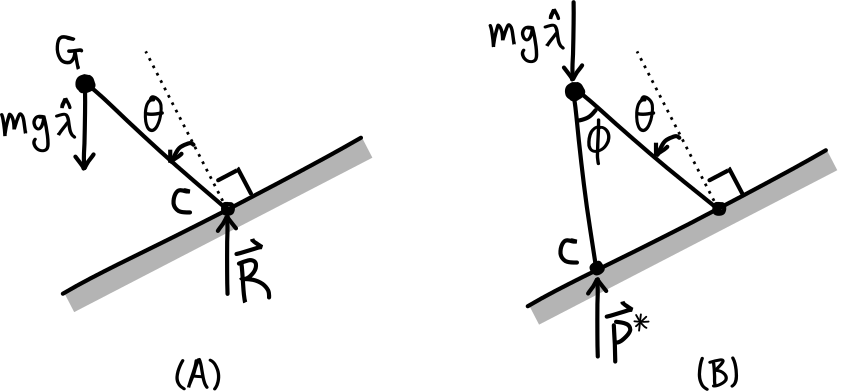
\includegraphics[width=0.7\textwidth]{Figures/RimlessSmoothAndCollision}\par
\end{centering}
\caption[Diagram: Rimless Wheel Free Body Diagrams]{Rimless wheel free body diagrams. Diagram (A) is a free body diagram for the smooth ``flight'' of the wheel. Diagram (B) is a free body diagram for the spoke collision of the wheel.}
\label{fig:RimlessSmoothAndCollision}
\end{figure}
%

The angular momentum before collision $n+1$ is

\begin{equation}
\vec{\mathbf{H}}_{/C,n+1}^{-} = \vec{\mathbf{r}}_{G/C} \times \vec{\mathbf{v}}_{G}^{-} + I \omega_{n+1}^{-} \vec{\mathbf{k}}
\label{eq:RimlessHMinus}
\end{equation}

The angular momentum after collision $n+1$ is

\begin{equation}
\vec{\mathbf{H}}_{/C,n+1}^{+} = (I + ml^{2} ) \omega_{n+1}^{+} \hat{\mathbf{k}}
\label{eq:RimlessHPlus}
\end{equation}

Here, the moment of inertia used is about point $C$. Accordingly, this moment of inertia is the sum of the centroidal moment of inertia and a term from the parallel axis formula. By equating these two momenta and expressing explicity all the terms in equation \ref{eq:RimlessHMinus}, the angular speed after the collision is given by

\begin{equation}
\omega_{n+1}^{+} = \frac{I + ml^{2} \cos{\phi}}{I + ml^2} \omega_{n+1}^{-}
\label{eq:RimlessOmegaPlus}
\end{equation}

A qualitative description of the rimless wheel motion is given by the graphs in figure \ref{fig:RimlessPlots}. Collision $n$ ends at $t = 0$ and collision $n+1$ starts at $t = t^*$. The wheel rotates quickly with $\omega = \omega_{n}^{+}$ right after the collision. Depending on $\phi$, the mass may come out of the collision before or at the apex of its ``flight'' path. If $\phi$ is sufficiently large, the mass slows down as its mass is elevated to the apex of the path. Otherwise, the mass starts its ``flight'' at the apex. The minimum angular speed is achieved at the apex of the smooth "flight". The wheel accelerates downward from its apex as the next spoke approaches collision. Just before the collision, the wheel rotates with angular speed $\omega = \omega_{n+1}^{-}$ (figure \ref{fig:RimlessPlots}b).

% FIGURE
\begin{figure}[h]		% h="here" t="top" b="bottom" p="separate page"
\begin{centering}
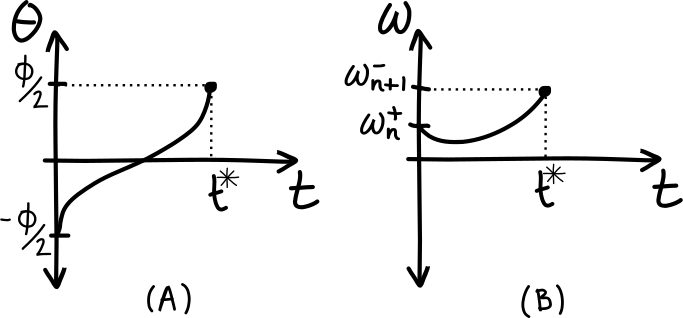
\includegraphics[width=0.7\textwidth]{Figures/RimlessPlots}\par
\end{centering}
\caption[Plot: Rimless Wheel State vs. Time for Smooth ``Flight'']{Rimless wheel state vs. time for smooth flight. Plot (A) shows the rotation of the wheel throughout the smooth ``flight'', up until the time $t^{*}$ when the collision occurs. The flight is defined as occuring between $\theta = -\phi/2$ and $\theta = \phi/2$. Plot (B) shows the angular speed throughout the smooth ``flight'', which starts at $\omega_{n}^{+}$ and ends at $\omega_{n+1^{-}}$.}
\label{fig:RimlessPlots}
\end{figure}
%
\begin{comment}
 The dip in the curve depends on the the spoke separation $\phi$.
\end{comment}

% FIGURE
\begin{figure}[h]		% h="here" t="top" b="bottom" p="separate page"
\begin{centering}
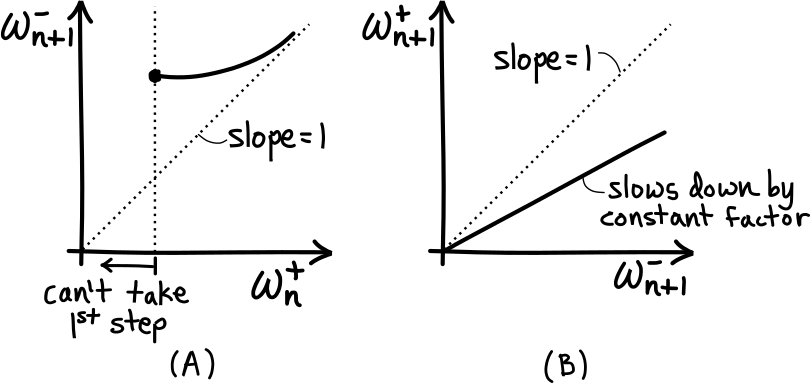
\includegraphics[width=0.7\textwidth]{Figures/RimlessPlots2}\par
\end{centering}
\caption[Plot: Rimless Wheel Angular Speed Relations]{Rimless wheel angular speed relations. Plot (A) provides $\omega_{n+1}^{-}$ at the end of the ``flight'' from $\omega_{n}^{+}$ from the beginning of the ``flight''. Plot (B) provides the angular speed after the collision $\omega_{n+1}^{+}$ from the angular speed before the collision $\omega_{n+1}^{-}$.}
\label{fig:RimlessPlots2}
\end{figure}
%
\begin{comment}
The curve asymptotically approaches $\omega_{n+1}^{-} = \omega_{n}^{+}$ as gravity has less time to accelerate the wheel for faster initial angular speeds. 
\end{comment}

The periodic evolution of the wheel's angular speed before and after collisions is described by figure \ref{fig:RimlessPlots2}. Figure \ref{fig:RimlessPlots2}a describes the change in angular speed between the beginning and end of the smooth flight. There is a threshold value below which continued motion is not possible and the wheel does not proceed continually down the incline. In this case the wheel does not have enough initial momentum to move through the apex of the smooth flight path. For greater initial speeds $\omega_{n}^{+}$ for a given cycle of the motion, the wheel starts the smooth flight with more momentum and thus finishes the flight with greater final speeds $\omega_{n+1}^{-}$. The curvature in this relation results from the fact that the force of gravity contributes less to the increased final speed as the initial speed increases. For large $\omega_{n}^{+}$ the flight occurs quickly enough that the downward acceleration due to gravity does not have the time to noticably increase the speed of the wheel.

Figure \ref{fig:RimlessPlots2}b picks up where figure \ref{fig:RimlessPlots2}a leaves off, literally. This figure provides the difference between the speed $\omega_{n+1}^{-}$ before the next collision and the speed $\omega_{n+1}^{+}$ after this collision. The angular speed of the wheel is discontinuous through the collision since the collision is not elastic. The slope of the straight line in figure \ref{fig:RimlessPlots2}b is given by the constant factor in equation \ref{eq:RimlessHPlus}. The slope here can be thought of as a coefficient of restitution.

The curves in these plots are dependent on the parameters of the spoked wheel model. For example, if $\gamma = 0$ then the incline becomes a flat surface and the motion is not as interesting as for the general case examined here. If $\gamma = 0$, the motion cannot be stable if the collisions are not perfectly elastic. 

% FIGURE
\begin{figure}[h]		% h="here" t="top" b="bottom" p="separate page"
\begin{centering}
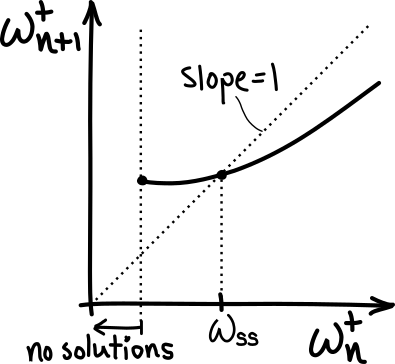
\includegraphics[width=0.3\textwidth]{Figures/RimlessStrideFunction}\par
\end{centering}
\caption[Plot: Rimless Wheel Stride Function]{Rimless wheel stride function. Provides the angular speed at the start of a ``flight'' from the angular speed at the start of the previous ``flight''. This figure is generated from a composition of the plots in figure \ref{fig:RimlessPlots2}. The point at which the curve intersects the $\omega_{n+1}^{+} = \omega_{n}^{+}$ line is a stable fixed point.}
\label{fig:RimlessStrideFunction}
\end{figure}
%

The composition of the graphs in figure \ref{fig:RimlessPlots2} yields figure \ref{fig:RimlessStrideFunction}, which is called a \emph{stride function}\index{stride function}. The stride function can be used to understand how the motion of the wheel evolves over numerous collisions. To determine the motion of the wheel, or $\omega_{n+1}$, throughout multiple cycles of its motion, use the following procedure with figure \ref{fig:RimlessStrideFunction}:

\begin{enumerate}
\item Choose an initial value $\omega_{0}^{+}$ on the $\omega_{n}^{+}$-axis.
\item Trace this point up to the thick curve. This point on the thick curve provides the value of $\omega_{1}^{+}$ on the vertical axis.
\item Now $n = 1$; find the value of $\omega_{1}^{+}$ on the horizontal axis by tracing horizontally from the vertical axis to the \textit{slope = 1} line.
\item Trace from the \textit{slope = 1} line to the thick line to discover the value of $\omega_{2}^{+}$ on the vertical axis.
\item Repeat.
\end{enumerate}

Again, the angular speed at the beginning of the smooth flight must surpass a threshold value. If the initial angular speed has the steady state value $\omega_{ss}$, the motion is steady and periodic. Note that the threshold angular speed, the steady state angular speed, and the shape of the curve in the figure are all functions of the model's parameters. Since the curve is increasing everywhere, all initial values of $\omega_n^+$ above the threshold cause $\omega_n^+$ to tend toward $\omega_{ss}$. That is, the system tends toward the stable fixed point $\omega_{ss}$ for the parameters used to generate figure \ref{fig:RimlessStrideFunction}.

\section{Spring Loaded Inverted Pendulum} %(notes page 27-30)
\label{sec:SpringLoadedInvertedPendulum}

To analyze the passive dynamics of the SLIP model presented in section \ref{sec:SLIP}, it is important to give careful thought to the construction of the Poincare map. Assume that the model travels with a periodic gait. There are peaks and valleys in the trajectory of the center of mass of the model, as shown in figure \ref{fig:SLIPSections}. The Poincare map can be constructed at various points along the trajectory, and some points are better than others. Remember that the Poincare map is constructed by sampling the parameters that describe the motion of the system once per period, and plotting those points. For the SLIP model of walking and running, the system can be fully described by four coordinates of the center of mass: $x$, $y$, $\dot{x}$, and $\dot{y}$. The contact angle of the leg, $\theta_{c}$, is considered to be an initial condition, and is not a part of the system state. Ideally, the Poincare map of the system would plot only two parameters. 

There are quite a few options for points along the gait cycle to construct a Poincare map. The point at which one ``slices'' the gait cycle is called a Poincare section. The point of choosing a section is to reduce the number of equations which we must solve to fully define the motion of the hopper. Six possible sections to choose are as follows:

\begin{enumerate}

\item Transition from stance to flight. Choosing this transition point allows the gait trajectory to be built from only two segments: a stance phase and a parabolic flight phase. 

\item Transition from flight to stance. No need to worry about $y=l_{0}\cos{\theta_{c}}$. Three section variables: $x$, $\dot{x}$, and $\dot{y}$.

\item Point of maximum height in flight: $\dot{y}=0$. Three section variables: $x$, $\dot{x}$, and $y$.
\label{item:MaxHeight}

\item Point of minimum height in stance: $\dot{y}=0$. Three section variables: $x$, $\dot{x}$, and $y$.

\item Point where the spring is maximally compressed. 

\item Point where the stance leg is vertical.

\end{enumerate}

% FIGURE
\begin{figure}[h]		% h="here" t="top" b="bottom" p="separate page"
\begin{centering}
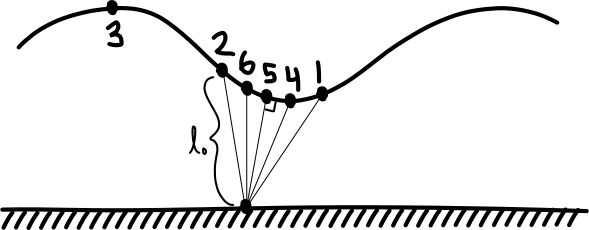
\includegraphics[width=0.6\textwidth]{Figures/SLIPSections}\par
\end{centering}
\caption[Diagram: SLIP Options for Poincare Sections]{SLIP options for Poincare sections. Various points in the gait cycle of the SLIP model can be used to generate a Poincare map. The section, or a particular slice of the periodic gait cycle, can fully define the motion. Each section is defined by a different occurence. Six different options are proposed, and option 3 is considered in more detail.}
\label{fig:SLIPSections}
\end{figure}
%

Though all of the options are valid, section \ref{item:MaxHeight} will be analyzed here in further detail. This section reduces the four-dimensional phase space $x$, $y$, $\dot{x}$, and $\dot{y}$ to a three dimensional section $x$, $\dot{x}$, and $y$ because it is known that $\dot{y} = 0$ at the section slice. Additionally, we don't need to know $x$ to be able to predict the motion of the center of mass because the center of mass is traveling in the x-direction, and it location relative to fixed the fixed x-axis is irrelevant if the motion is periodic. More formally, given $y_{n}$ and $\dot{x}_{n}$, we can predict $y_{n+1}$ and $x_{n+1}$, where $n$ is the number of times the section is repeated. 

Given the model and the free body diagram presented in section \ref{sec:SLIP}, the trajectory of the center of mass can be calculated with the use of MATLAB's ordinary differential equation (ODE) solvers like ode45.m or ode112.m. There are three distinct segments of motion for the chosen poincare section. The first is the parabolic flight from the top of the trajectory to where the leg initially touches the ground. This first segment's motion is described by one set of differential equations. The second segment of motion is the stance phase, where the spring is compressed. This segment is described by a different set of differential equations. Finally, the third segment is again parabolic flight, described by the same differential equations as the first segment. When writing code to simulate the flight, one can recognize the transitions with the event detection feature of MATLAB's ODE solvers. 

In the world of Legged Locomotion, it is important to analyze the stability of locomotion models. To analyze the stability of the SLIP model, it is necessary to develop a stride function, or return map, that describes how the center of mass goes from $y_{n}$ and $\dot{x}_{n+1}$ to $y_{n+1}$ and $\dot{x}_{n+1}$. For clarity in this analysis, define $q_{1}\equiv y_{n}$ and $q_{2}\equiv\dot{x}_{n}$. Where, $q$ is a vector of the two states $q_{1}$ and $q_{2}$, and $q_{n+1}$ is a function of $q$ called $f(q)$. A full expansion of this function reveals that it is made up of two functions that each act on $q$:

\begin{align}
q_{1,n+1}= f_{1}(q_{1,n},q_{2,n}) \notag \\
q_{2,n+1}=  f_{2}(q_{1,n},q_{2,n})
\label{eq:FullFunctionDefinition}
\end{align}

For a given $q_{n}=[q_{1,n},q_{2,n}]$, the fixed point that describes periodic motion occurs when $q_{n}=f(q_{n})=q_{n+1}$. The fixed point can be found using similar methods as were used to find the fixed point for the rimless wheel. However for this problem, the calculations will be performed in two dimensions, not one.

Given some kind of simulation that uses MATLAB's ODE solvers to calculate the trajectory of the center of mass, values for $q_{n}$ and $q_{n+1}$ can be obtained, and a function $f$can be built that returns $q_{n+1}=f(q_{n})$. Given such a function $f$, the fixed point can be solved for by using MATLAB's fsolve.m. However, fsolve.m requires that the problem take the form $g(q)=0$, so it is helpful to define a function $g(q)\equiv f(q)-q$. For periodic motion, the goal is to solve for $q$ such that $g(q)=0$. This solution is called the ``root'' and will be referred to here as $q^{*}$.

 \begin{align}
 \begin{bmatrix}
 f_{1}(q_{1},q_{2}) \\
 f_{2}(q_{1},q_{2})
 \end{bmatrix}
 -
 \begin{bmatrix}
 q_{1} \\
 q_{2}
 \end{bmatrix}
 =
 \begin{bmatrix}
 0 \\
 0
\end{bmatrix}
\label{eq:GDefinition}
\end{align}


After solving equation \ref{eq:GDefinition}, it's desirable to know if the motion is stable near this fixed point. To assess the stability of the fixed point $q^{*}$, the function $f(q)$, must first be linearized about $q^{*}$. This can be done with the first two terms of a Taylor expansion:

\begin{equation}
f ( q ) = f ( q^{*} ) + f' |_{q^{*}} ( q - q^{*} ) + ...
\label{eq:LinearShorthand}
\end{equation}

If the function $f(q)$ is expanded to its full two-parameter form, a matrix called the Jacobian, $J$, reveals itself. By examining the expanded form of the function $f(q)$, it is easy to see why the Jacobian determines the stability of the motion determined by $f(q)$:

\begin{align}
\begin{bmatrix}
f_{1} (q_{1},q_{2}) \\
f_{2} (q_{1},q_{2}) 
\end{bmatrix}
=
\begin{bmatrix}
q_{1}^{*} \\
q_{2}^{*}
\end{bmatrix}
+
\begin{bmatrix}
\frac{\partial f_{1}}{\partial q_{1}} &  \frac{\partial f_{1}}{\partial q_{2}} \\
\frac{\partial f_{2}}{\partial q_{1}} & \frac{\partial f_{2}}{\partial q_{2}}
\end{bmatrix}
\begin{bmatrix}
\epsilon_{1} \\
\epsilon_{2}
\end{bmatrix}
+
...
\label{eq:LinearLonghand}
\end{align}

For the motion to be periodic, it's already been shown that $f(q)$ must equal $q^{*}$. Any time a given step $q$ is given as input to the return map $f(q)$, the return map must output the input. The q that accomplishes this is called $q^{*}$ by definition. If the input $q$ deviates from this ideal $q^{*}$ and causes $f(q)$ to output something other than the input $q$, the motion is considered stable if it eventually returns the ideal $q^{*}$ after multiple iterations. 

This can be seen by examining the second term on the right side of equation \ref{eq:LinearLonghand}, where $\epsilon_{1}$ is the error associated with $q_{1}$ and $\epsilon_{2}$ is the error associated with $q_{2}$. These errors $\epsilon_{1}$ and $\epsilon_{2}$ represent a disturbance introduced by variation in terrain or environment of the hopping robot. Every time the robot goes through one gait cycle, the errors $\epsilon$ will change from the initial disturbance $\epsilon_{0}$, based on the difference between the output of $f(q)$ and $q^{*}$ and the values of the elements in the Jacobian, $J$. Though the values of the elements of the Jacobian do not change with each step, the change in the values of the errors $\epsilon$ causes the value of the second term of the right side of equation \ref{eq:LinearLonghand} to either shrink or grow with each step. If the errors $\epsilon$ grow, so does the second term of the right side of equation \ref{eq:LinearLonghand}, and the motion of the hopper is unstable. So the important question is: does the initial perturbation $\epsilon_{0}$ grow? This can be determined by just examining the product of the Jacobian and the perturbation vector $\epsilon_{n}$:

\begin{align}
\begin{bmatrix}
\epsilon_{1,n+1} \\
\epsilon_{2,n+1}
\end{bmatrix}
=
\begin{bmatrix}
J_{11} &  J_{12} \\
J_{21} &  J_{22} 
\end{bmatrix}
\begin{bmatrix}
\epsilon_{1,n} \\
\epsilon_{2,n}
\end{bmatrix}
\label{eq:ErrorAndJacobian}
\end{align}

In equation \ref{eq:ErrorAndJacobian} the subscripts denote the associated element of $f(q)$. In the following analysis, the subscripts denote the iteration of the perturbation vector. It's clear that $\epsilon_{1}=J\epsilon_{0}$ and $\epsilon_{2}=J\epsilon_{1}=JJ\epsilon_{0}$. It follows then that $\epsilon_{n}=J\epsilon_{n-1}=J^{n}\epsilon_{0}$. The goal here is to find out if $\epsilon_{n}$ decays to zero as $n$ reaches infinity. If that is true, then the hopper is stable. By making use of the eigenvector definition, the value of $\epsilon_{n}$ as $n$ reaches infinity can be found:

\begin{equation*}
J\vv=\lambda\vv 
\end{equation*}

Given that for this problem, $J$ will always be a two-by-two matrix, it is also true that there will always be two eigenvalues $\lambda$ and two corresponding eigenvectors that satisfy the eigenvector definition:

\begin{align*}
J\epsilon=&J(a_{1}\vv_{1}+a_{2}\vv_{2}) \\
=&a_{1}\lambda_{1}\vv_{1}+a_{2}\lambda_{2}\vv_{2}
\end{align*}

Now, replacing $J$ with $J^{n}$ gives the following:

\begin{equation*}
J^{n}\epsilon=\lambda_{1}^{n}a_{1}\vv_{1}+\lambda_{2}^{n}a_{2}\vv_{2}
\end{equation*}

which decays as $n$ reaches infinity for all $a_{1}$ and $a_{2}$ only if $|\lambda_{1}| < 1$ and $|\lambda_{2}| < 1$.

There are a few different ways to find the Jacobian, $J$. The easiest way to find the Jacobian is to have a root-finding program, such as MATLAB's fsolve.m, output the Jacobian when it finds the root $q^*$. Another way is to refer to equation \ref{eq:LinearLonghand} and find the partial derivatives like so:

\begin{equation}
\lim_{h \to 0} \frac{y(x+h)y(x)}{h}=\frac{\partial y}{\partial x}\bigg|_{x^{*}}
\label{eq:FindingJacobian}
\end{equation}

Finally, one could find $J$ by using an infinitesimally small value $\delta$ to approximate the partial derivatives in \ref{eq:FindingJacobian}, like so: 

\begin{equation}
J= \frac{1}{\delta}
\begin{bmatrix}
f_{1}\left(q^{*}+\begin{bmatrix} \delta \\ 0 \end{bmatrix}\right) - f_{1}(q^{*}) & f_{1}\left(q^{*}+\begin{bmatrix} 0 \\ \delta \end{bmatrix}\right) - f_{1}(q^{*}) \\[3mm]
f_{2}\left(q^{*}+\begin{bmatrix} \delta \\ 0 \end{bmatrix}\right) - f_{2}(q^{*}) & f_{2}\left(q^{*}+\begin{bmatrix} 0 \\ \delta \end{bmatrix}\right) - f_{2}(q^{*})
\end{bmatrix}
\label{eq:FindingQStar}
\end{equation}

In summary, there are three steps involved in answering the question of stability with the hopping robot. First, find $q^*$ accurately. Second, find the Jacobian $J$. Third, find the eigenvalues of $J$.


\section{Simplest Walker} % (notes page 31-34)
\label{sec:SimplestWalker}
\index{simplest walker}



The rimless wheel model described in section \ref{sec:RimlessWheel} can be modified logically in order to create a model of a simple bipedal gait. With the rimless wheel, only two spokes at any given time are involved in the interesting dynamics of the motion. Naturally, these two spokes can be thought of as simple legs. In fact, Garcia \cite{garcia97} asserts that this model is the simplest (irreducible) model of walking. As figure \ref{fig:SimplestWalkerPendulum} hints, this model is a simplification of a double-pendulum model that was studied by 
others in the 1980's. Indeed, this model contains two single-pendula.

% FIGURE
\begin{figure}[h]		% h="here" t="top" b="bottom" p="separate page"
\begin{centering}
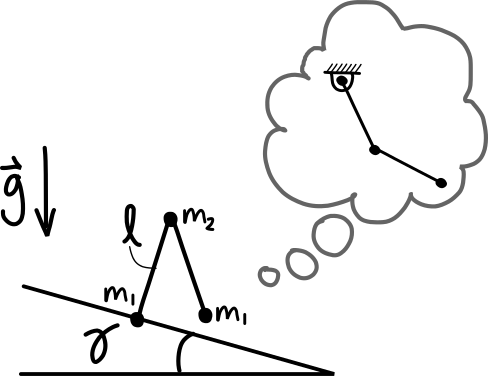
\includegraphics[width=0.5\textwidth]{Figures/SimplestWalkerPendulum}\par
\end{centering}
\caption[Diagram: Simplest Walker Model]{Simplest walker model. This model consists of only two massless links of length $l$ joined at the hip, with masses $m_{1}$ and $m_{2}$ at the ends of the links. For certain slopes of the incline $\gamma$, stable motion is possible.}
\label{fig:SimplestWalkerPendulum}
\end{figure}
%

Similar to the rimless wheel model, the locomotive is traverseing an incline defined by the angle $\gamma$. The leg that is in no-slip contact with the incline is called the \textit{stance leg} and the other leg is called the \textit{swing leg}\index{stance leg}\index{swing leg}. The legs of length $l$ are massless, the mass of the hips is $m_{2}$, and the mass of each foot is $m_{1}$, with $\beta = m_{1} / m_{2} \ll 1$.

% FIGURE
\begin{figure}[h]		% h="here" t="top" b="bottom" p="separate page"
\begin{centering}
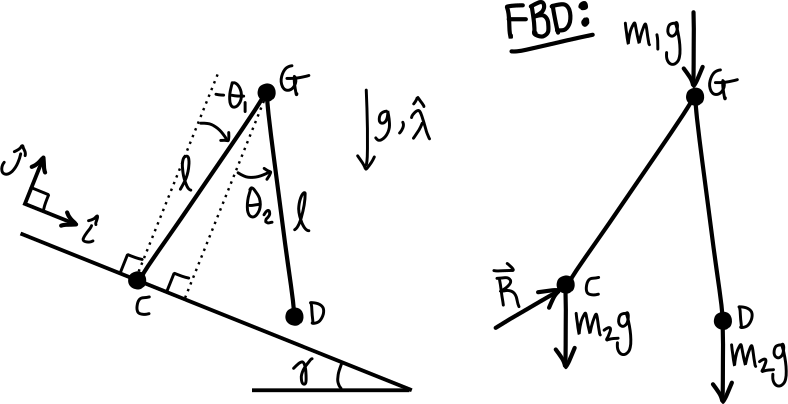
\includegraphics[width=0.8\textwidth]{Figures/SimplestWalkerFBD}\par
\end{centering}
\caption[Diagram: Simplest Walker Free Body Diagram]{Simplest walker free body diagram. The configuration of the model is defined by the rotations $\theta_{1}$ and $\theta_{2}$. Weights act at all three masses, and a ground reaction force acts at the contact point $C$.}
\label{fig:SimplestWalkerFBD}
\end{figure}
%

Unlike the rimless wheel, this system has two degrees of freedom because the angle between the legs is not fixed. The configuration of the locomotive is defined by the angles $\theta_1$ and $\theta_2$ and the corresponding angular speeds $\dot{\theta}_1$ and $\dot{\theta}_2$. Both angles are defined with respect to the normal of the incline. The free body diagram of the model in figure \ref{fig:SimplestWalkerFBD} describes this locomotive in more detail. The forces present in the full system are the weight of each mass and the reaction force of the incline against the stance leg (the vector sum of static friction and normal force). The motion proceeds under the force of gravity. A free body diagram of the swing leg (not shown) would reveal a force in the swing leg that is required to maintain the joint constraint at point $G$. This force is decomposed into two components: tension $T$ along the leg and a force $F$ perpendicular to the leg. 

\begin{comment}
[chris: in Alan's notes where is F's line of action?]
\end{comment}

There are six unknowns in this model: the angular acceleration of each degree of freedom, $\ddot{\theta}_{1}$ and $\ddot{\theta}_{2}$, the tension $T$ and perpendicular force $F$ in the swing leg, and the two components of the support force $\vec{\mathbf{R}}$. The system is described by two free body diagrams and three momentum balances for each diagram. This gives six equations with which to solve for all six unknowns. To obtain only the motion of the locomotive and avoid the support forces and internal forces, only angular momentum balance is required for each of the two free body diagrams. For the system free body diagram angular momentum balance about $C$ yields

\begin{align}
\Sigma \vM_{/C} &= \vHdot_{/C} \notag \\
(\vr_{G/C} \times m_{1} g  \ul ) + (\vr_{D/C} \times m_{2} g  \ul ) &= (\vr_{G/C} \times m_{1} \va_{G}) + (\vr_{D/C} \times m_{2} \va_{D})
\label{eq:SimplestWalkerAMB1}
\end{align}

where $ \ul $ is directed downward, in the direction of gravity.

Likewise, angular momentum balance of just the swing leg about $G$ yields

\begin{align}
\Sigma \vM_{/G} &= \vHdot_{/G} \notag \\
\vr_{D/G} \times m_{2} g  \ul  &= \vr_{D/G} \times m_{2} \va_{D}
\label{eq:SimplestWalkerAMB2}
\end{align}

To solve these equations, expressions for $\vec{\mathbf{a}}_{G}$ and $\vec{\mathbf{a}}_{D}$ are required.

\begin{align}
\va_{G} &= -\dot{\theta}_{1}^{2} \vr_{G/C} + \ddot{\theta}_{1} \uk \times \vr_{G/C} \\
\va_{D}  &= \va_{G} + \va_{D/G} \notag \\
 &= \va_{G}  -\dot{\theta}_{2}^{2} \vr_{D/G} + \ddot{\theta}_{2} \uk \times \vr_{D/G}
\end{align}

where $\vr_{G/C} = l (- \sin{\theta_{1}} \ui +\cos{\theta_{1}} \uj)$ and $\vr_{G/C} = l (\sin{\theta_{2}} \ui - \cos{\theta_{2}} \uj)$. The equations can be greatly simplified if the feet have no mass, $\beta = 0$.


As with the rimless wheel, equations \ref{eq:SimplestWalkerAMB1} and \ref{eq:SimplestWalkerAMB2} describe the dynamics of the model during the smooth ``flight''. The solution for the smooth flight motion requires information about the plastic collision that occurs between flights. The instant at which the collision starts is called \textit{heelstrike}\index{heelstrike}. At heelstrike, point $C$ collides with the incline and the collision is analyzed by the following equalities across the collisions

\begin{align}
\vHdot_{/C}^{+} &= \vHdot_{/C}^{-} \notag \\
\vHdot_{/G}^{+} &= \vHdot_{/G}^{-} \notag
\label{eq:SimplestWalkerCollision}
\end{align}

These equations result in expressions that are very similar to equations \ref{eq:RimlessHPlus} and \ref{eq:RimlessHMinus} for the rimless wheel, except that this time there are two degrees of freedom to manage. As for the rimless wheel, the weight of the masses can be ignored in the angular momentum expressions since the collisions occur so quickly. The coupled differential equations for $\theta_{1}$ and $\theta_{2}$ and the collision equations are presented in \cite{garcia97}. 

The equations of motion in this model are actually \emph{nonlinear}\index{nonlinear}. This means that for certain system parameters the motion of the locomotive is chaotic, and small changes in initial conditions result in largely different motions. The model exhibits \emph{period-doubling}\index{period-doubling} phenomena as the angle of the incline $\gamma$ is increased. The period-doubling is captured in the Poincare map\index{Poincare map} in figure \ref{fig:SimplestWalkerEigenvalues}.

A Poincare map is a graph in which the value of a state variable of the model in each cycle of the motion is plotted as a function of some parameter of the model. The natural parameter to use in this case is the angle of the incline $\gamma$. The vertical axis of the Poincare map holds the step length for each gait cycle. For small inclines, the step length is constant for each gait cycle and so there is only one curve to the left of the first point where the curve splits into two curves at what is called a \emph{bifurcation point}\index{bifurcation point}.

% FIGURE
\begin{figure}[h]		% h="here" t="top" b="bottom" p="separate page"
\begin{centering}
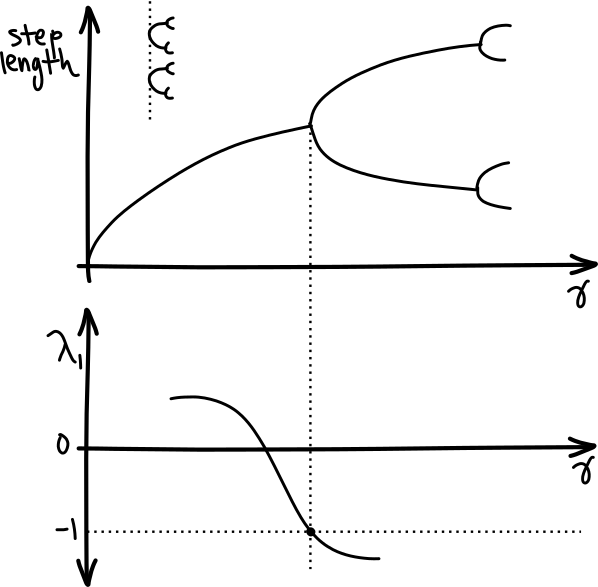
\includegraphics[width=0.6\textwidth]{Figures/SimplestWalkerEigenvalues}\par
\end{centering}
\caption[Plot: Simplest Walker Bifurcation and Eigenvalues]{Simplest walker bifurcation and eigenvalues. The top plot is a bifurcation diagram that shows the step length for many gait cycles for a given value of $\gamma$, as $\gamma$ is varied. The bottom plot shows the first eigenvalue of the Jacobian of the system's Poincare map (map not shown). Eigenvalues of $\lambda = -1$ correspond to bifurcation points in the top plot, and \emph{period-doubling}: beyond $\gamma = 0.015 rad$, the simplest walker executes a limping period-2 gait in which step length alternates between two values for each period.}
\label{fig:SimplestWalkerEigenvalues}
\end{figure}
%

The nonlinear behavior of the model is determined by the Jacobian of the Poincare map. The first eigenvalue $\lambda$ of this Jacobian follows the curve presented in figure \ref{fig:SimplestWalkerEigenvalues}. The values of $\gamma$ for which the eigenvalue $\lambda = -1$ are the incline angles at which bifurcation occurs. After this bifurcation point, the motion is described as being \textit{period-2}. This means that the step length oscillates between two values between gait cycles. This motion resembles limping, in which one leg takes larger steps than the other.

For $0 < \gamma < 0.015$ rad, the motion of the simplest walker model is stable. The fact that such a simple mechanical model of locomotion has stable solutions without actuation or control hints that the coordination of locomotion is mostly mechanical. This view is in constrast with a view that states coordination results from muscle action or from neurological control \cite{garcia97}.

For an in-depth description of the nonlinear behavior of this model, 
refer to Garcia \cite{garcia97}.




All the models presented in this chapter and chapter \ref{sec:ModelingLeggedLocomotion} are very simple. Mass has been concentrated at the hip or at the foot. More detailed dynamic models of locomotion can be developed in a somewhat logical fashion. The models can be extended by including distributed masses for the legs, or perhaps links for the upper body. For these situations, analytical descriptions quickly become cumbersome. It is important though to examine if such detailed models add any new information or provide any additional accuracy. There is an elegance to the ability to make important conclusions about animal locomotion from only the motion of a few point masses.


\begin{comment}
-eigenvalues less than one means stability.
-describe poincare/stability
-detail that dHdt vs Hdot only if C is not moving
-didnt talk about the passive nature of the locomotion
\end{comment}
